% Author: Matúš Fignár
% Date: 4.4.2024
% 3. project for Typografie a publikování VUT FIT BRNO

\documentclass[11pt, a4paper]{article}
\usepackage[left=2cm, top=3cm, text={170mm, 240mm}]{geometry}
\usepackage[utf8]{inputenc}
\usepackage[czech]{babel}
\usepackage[T1]{fontenc}
\usepackage{times}
\usepackage[linesnumbered,czech,ruled]{algorithm2e}
\usepackage[hidelinks]{hyperref}
\usepackage{multirow}
\usepackage{graphicx}
\usepackage{tikz}
\usepackage{pdflscape}



\begin{document}
\begin{titlepage}
    \begin{center}
        \textsc{\Huge{Vysoké učení technické v~Brně\\[0.4em]}
        \huge{Fakulta informačních technologií}}\\        
        \vspace{\stretch{0.382}}
        \LARGE{Typografie a~publikování\,--\,3. projekt}\\
        \Huge{Tabulky a~obrázky}\\
        \vspace{\stretch{0.618}}
    \end{center}
    \Large{\today\hfill Matúš Fignár}
\end{titlepage}

\section{Úvodní strana}
Název práce umístěte do zlatého řezu a~nezapomeňte uvést \emph{dnešní} (today) datum a~vaše jméno a~příjmení.

\section{Tabulky}
Pro sázení tabulek můžeme použít buď prostředí\texttt{ tabbing }nebo prostředí\texttt{ tabular}.

\subsection{Prostředí\texttt{ tabbing}}
Při použití\texttt{ tabbing }vypadá tabulka následovně:
\begin{tabbing}
    Vodní melouny \quad \= Množství \hspace{3pt} \= Jednotka \quad \= cena za jedn. \quad\:\=  .\kill
    \textbf{Ovoce} \> \textbf{Množství} \> \textbf{Jednotka} \> \textbf{Cena za jedn.} \> \textbf{Cena celková} \\
    Jablka \> 3 \> kg \> 25,90\,Kč \> 77,70\,Kč \\
    Hrušky \> 2,5 \> kg \> 27,40\,Kč \> 68,50\,Kč \\
    Vodní melouny \> 1 \> kus \> 35,\textendash\,Kč\> 35,\textendash\,Kč \\
\end{tabbing}

\noindent Toto prostředí se dá také použít pro sázení algoritmů, ovšem vhodnější je použít prostředí\texttt{ algorithm }nebo\texttt{ algorithm2e }(viz sekce \ref{sec:algoritmy}).

\subsection{Prostředí\texttt{ tabular}}
Další možností, jak vytvořit tabulku, je použit prostředí\texttt{ tabular}. Tabulky pak budou vypadat 
takto\footnote{Kdyby byl problém s\texttt{ cline,} zkuste se podívat třeba sem: \href{http://www.abclinuxu.cz/tex/poradna/show/325037}{http://www.abclinuxu.cz/tex/poradna/show/325037}}:
\\
\begin{table}[ht]
    \catcode`\-=12
    \begin{center}
        \begin{tabular}{|l|r|r|} \hline
            & \multicolumn{2}{c|}{\textbf{Cena}} \\
            \cline{2-3}
            \textbf{Měna} & \textbf{nákup} & \textbf{prodej} \\
            \hline
            EUR & 23{,}26 & 24{,}93 \\
            GBP & 29{,}56 & 29{,}83 \\
            USD & 22{,}27 & 23{,}12 \\
            \hline
        \end{tabular}
        \caption{Tabulka kurzů k~dnešnímu dni\label{tab:kursy}}
    \end{center}
\end{table}

\begin{table}[ht]
    \catcode`\-=12
    \begin{center}
        \begin{tabular}{|c|c|} \hline
            $A$ & $\neg A$ \\ \hline
            \textbf{P} & N \\ \hline
            \textbf{O} & O \\ \hline
            \textbf{X} & X \\ \hline
            \textbf{N} & P \\ \hline
        \end{tabular}
        \begin{tabular}{|c|c|c|c|c|c|} \hline
            \multicolumn{2}{|c|}{\multirow{2}{*}{$A \land B$}} & \multicolumn{4}{c|}{\textbf{$B$}} \\ \cline{3-6}
            \multicolumn{2}{|c|}{} & \textbf{P} & \textbf{O} & \textbf{X} & \textbf{N} \\ \hline
            \multirow{4}{*}{\textbf{$A$}} & \textbf{P} & P & O & X & N \\ \cline{2-6}
            & \textbf{O} & O & O & N & N \\ \cline{2-6}
            & \textbf{X} & X & N & X & N \\ \cline{2-6}
            & \textbf{N} & N & N & N & N \\ \hline
        \end{tabular}
        \begin{tabular}{|c|c|c|c|c|c|} \hline
            \multicolumn{2}{|c|}{\multirow{2}{*}{$A \lor B$}} & \multicolumn{4}{c|}{\textbf{$B$}} \\ \cline{3-6}
            \multicolumn{2}{|c|}{} & \textbf{P} & \textbf{O} & \textbf{X} & \textbf{N} \\ \hline
            \multirow{4}{*}{\textbf{$A$}} & \textbf{P} & P & P & P & P \\ \cline{2-6}
            & \textbf{O} & P & O & P & O \\ \cline{2-6}
            & \textbf{X} & P & P & X & X \\ \cline{2-6}
            & \textbf{N} & P & O & X & N \\ \hline
        \end{tabular}
        \begin{tabular}{|c|c|c|c|c|c|} \hline
            \multicolumn{2}{|c|}{\multirow{2}{*}{$A \rightarrow B$}} & \multicolumn{4}{c|}{\textbf{$B$}} \\ \cline{3-6}
            \multicolumn{2}{|c|}{} & \textbf{P} & \textbf{O} & \textbf{X} & \textbf{N} \\ \hline
            \multirow{4}{*}{\textbf{$A$}} & \textbf{P} & P & O & X & N \\ \cline{2-6}
            & \textbf{O} & P & O & P & O \\ \cline{2-6}
            & \textbf{X} & P & P & X & X \\ \cline{2-6}
            & \textbf{N} & P & P & P & P \\ \hline
        \end{tabular}
    \caption{Protože Kleeneho trojhodnotová logika už je \uv{zastaralá}, uvádíme si zde příklad čtyřhodnotové logiky\label{tab:logika}}
\end{center}
\end{table}
\pagebreak

\section{Algoritmy\label{sec:algoritmy}}
Pokud budeme chtít vysázet algoritmus, můžeme použít prostředí 
\texttt{algorithm}\footnote{\href{http://ftp.cstug.cz/pub/tex/CTAN/macros/latex/contrib/algorithms/algorithms.pdf}{http://ftp.cstug.cz/pub/tex/CTAN/macros/latex/contrib/algorithms/algorithms.pdf}}
nebo \texttt{algorithm2e}\footnote{\href{http://ftp.cstug.cz/pub/tex/CTAN/macros/latex/contrib/algorithm2e/doc/algorithm2e.pdf}{http://ftp.cstug.cz/pub/tex/CTAN/macros/latex/contrib/algorithm2e/doc/algorithm2e.pdf}}.\par
\noindent Příklad použití prostředí\texttt{ algorithm2e }viz Algoritmus \ref{alg:fastslam}.\\\bigskip

\IncMargin{1.5em}
\begin{algorithm}[H]\label{alg:fastslam}
\SetAlgoLined
\SetAlgoNoLine
\SetAlgoNlRelativeSize{-1}
\SetKwFor{For}{for}{do}{end\,for}
\DontPrintSemicolon
\SetNlSty{}{}{:}
\Indm\Indmm
\KwIn{$(X_{t-1}, u_t, z_t)$}
\KwOut{$X_t$}
\Indp\Indpp
$\overline{X_t} = X_t = 0$\;
\For{$k = 1$ \emph{to} $M$}{
    \Indpp
    $x_t^{[k]} = \emph{sample\_motion\_model}(u_t, x_{t-1}^{[k]})$\;
    $\omega_t^{[k]} = \emph{measurement\_model}(z_t, x_t^{[k]}, m_{t-1})$\;
    $m_t^{[k]} = updated\_occupancy\_grid(z_t, x_t^{[k]}, m^{[k]}_{t-1})$\;
    $\overline{X_t} = \overline{X_t} + \langle x^{[m]}_x, \omega^{[m]}_t \rangle$\;
    \Indmm
}
\For{$k = 1$ \emph{to} $M$}{
    \Indpp
    draw $i$ with probability $\approx \omega_t^{[i]}$\;
    add $\langle x^{[k]}_x, m^{[k]}_t \rangle$ to $X_t$\;
    \Indmm
}
\KwRet{$X_t$}\;
\caption{\textsc{FastSLAM}}
\end{algorithm}
\vspace{1.1em} 

\section{Obrázky}
Do našich článků můžeme samozřejmě vkládat obrázky. Pokud je obrázkem fotografie, můžeme klidně použít
bitmapový soubor. Pokud by to ale mělo být nějaké schéma nebo něco podobného, je dobrým zvykem takovýto
obrázek vytvořit vektorově.\par
\begin{figure}[h]
    \begin{center}
        \scalebox{0.4}{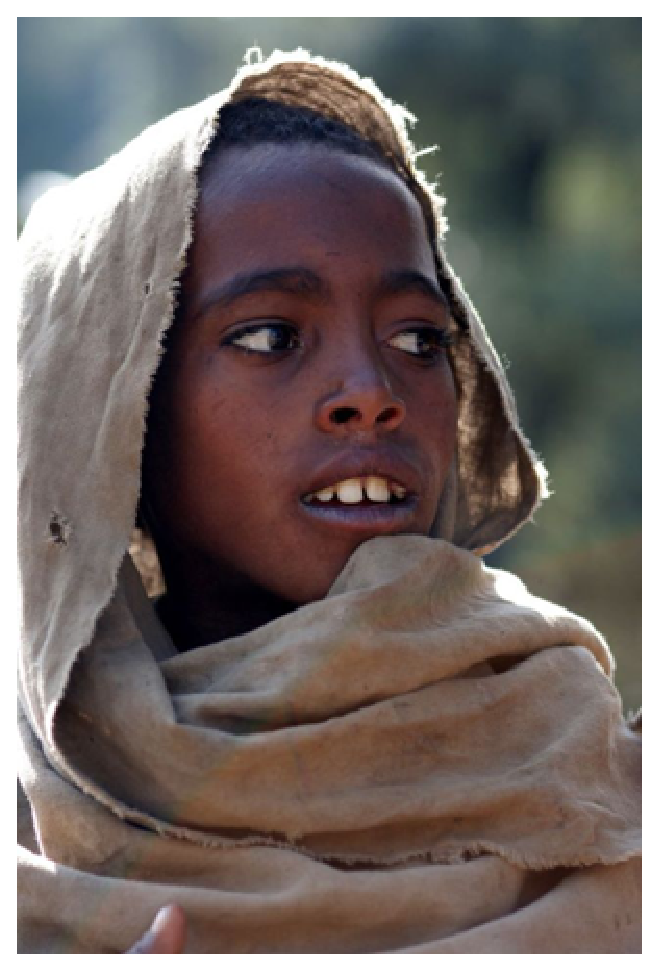
\includegraphics{etiopan.eps} \reflectbox{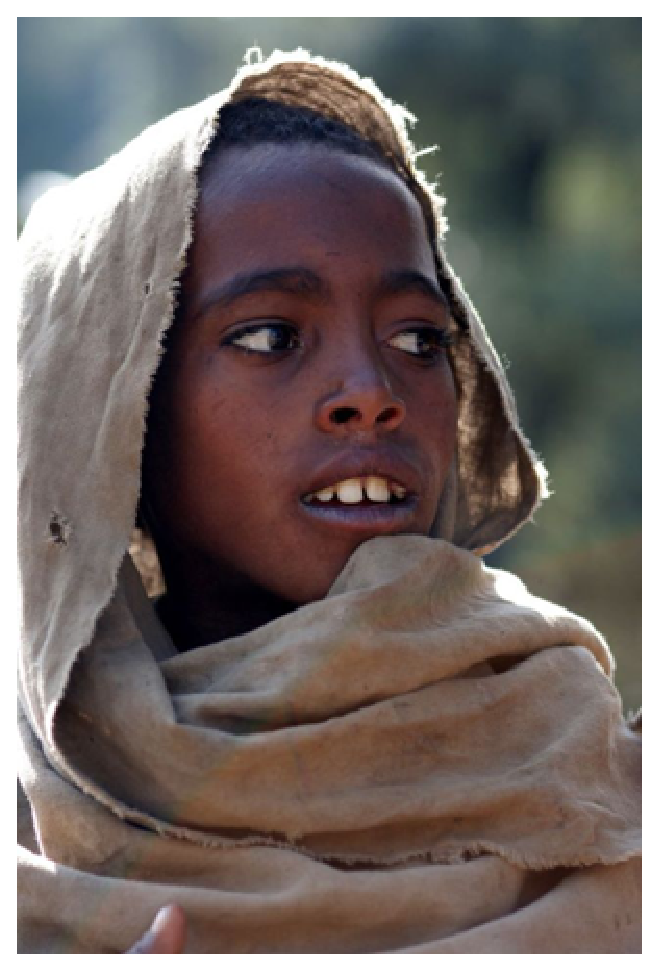
\includegraphics{etiopan.eps}}}
        \caption{Malý Etiopánek a~jeho bratříček\label{fig:etiopan}}
    \end{center}
\end{figure}
\bigskip
\pagebreak

Rozdíl mezi vektorovým\dots
\begin{figure}[h]
    \begin{center}
        \scalebox{0.4}{
\includegraphics{oniisan.eps}}
        \caption{Vektorový obrázek\label{fig:oniisan}}
    \end{center}
\end{figure}
\\
\noindent \dots~a bitmapovým obrázkem
\begin{figure}[h]
    \begin{center}
        \scalebox{0.6}{
\includegraphics{oniisan2.eps}}
        \caption{Bitmapový obrázek\label{fig:oniisan2}}
    \end{center}
\end{figure}

\noindent se projeví například pri zvětšení. \par
Odkazy (nejen ty) na obrázky \ref{fig:etiopan}, \ref{fig:oniisan} a \ref{fig:oniisan2}, na tabulky \ref{tab:kursy} a \ref{tab:logika} a také na algoritmus \ref{alg:fastslam} jsou udělány pomocí křížových \par
\noindent odkazů. Pak je ovšem potřeba zdrojový soubor přeložit dvakrát.\par
Vektorové obrázky lze vytvořit i přímu v \LaTeX{}u, například pomocí prostředí\texttt{ picture.}

\begin{landscape}
\begin{figure}[h]

    \begin{center}
        \begin{tikzpicture}[line width=1pt, scale=0.5]
            % fasáda 
            \draw (0, 1) -- (-1.5, 1) -- (-1.5, 15) -- (0, 16) -- (0, 17) -- (-2, 15.5) -- (-2, 15) -- (-1.5, 15); 
            \draw (0,0) -- (12, 0) -- (12, 25) -- (0, 21.5) -- (0, 0);
            \draw (12, 1) -- (25,1) -- (25, 10) -- (12,10); 
            \draw (23, 10) -- (23, 14) -- (12,14);
            \draw (23, 14) -- (23.5, 14.5) -- (12, 14.5);
            \draw (23.5, 14.5) -- (23.5, 15.5) -- (12, 21);
            \draw (12, 22) -- (25.5, 15.5) -- (23, 12.5);
            \draw (25.5, 15.5) -- (25.5, 16.5) -- (12, 23);

            % dvere
            \draw (3.5, 0) -- (3.5, 7) -- (8, 7) -- (8, 0);
            \draw (4, 1.5) -- (4, 6) -- (7, 6) -- (7, 1.5) -- (4, 1.5);
            \draw (4, 3) -- (7, 3);
            \draw (4, 4.5) -- (7, 4.5);
            \draw (7.5, 3.5) circle (0.25);

            % okna
            \draw (3.5, 9) -- (3.5, 19) -- (8, 20.3) -- (8, 9) -- (3.5, 9);
            \draw (4, 9) -- (4, 19.1) -- (4.2, 19.15) -- (4.2, 9);
            \draw (4.8, 9) -- (4.8, 19.4) -- (5, 19.45) -- (5, 9); 
            \draw (5.6, 9) -- (5.6, 19.65) -- (5.8, 19.7) -- (5.8, 9);
            \draw (6.4, 9) -- (6.4, 19.85) -- (6.6, 19.9) -- (6.6, 9);
            \draw (7.2, 9) -- (7.2, 20.05) -- (7.4, 20.1) -- (7.4, 9);
            \draw (14,10) -- (14, 13.5) -- (21, 13.5) -- (21,10);
            \draw (14.5, 10) -- (14.5, 13) -- (20.5, 13) -- (20.5,10);
            \draw (17.25, 10) -- (17.25,13) -- (17.75, 13) -- (17.75,10);

            % garaz
            \draw (13.5, 1) --  (13.5, 7.5) -- (22.5, 7.5) -- (22.5, 1);
            \draw[line width=1.8pt] (13.5, 6) -- (22.5, 6);
            \draw (13.5, 4.5) -- (22.5, 4.5);
            \draw (13.5, 3) -- (22.5, 3);
            \draw (13.5, 1.5) -- (22.5, 1.5);
            
            
            % dekorativne prvky a detaily
            \draw (11, 0) -- (11, 24.7);
            \foreach \y in {0, 0.5,...,24.5}{
                \draw (11, \y) -- (12, \y);
            }

            \draw (23.5, 15) -- (25, 15);
            \draw (21.45, 16.5) -- (22, 17.2);
            \draw (18.5, 17.9) -- (18.9, 18.65);

            % slnko
            \draw (25,25) circle (2);
            

        \end{tikzpicture}
        \caption{Vektorový obrázek moderního bydlení vhodného pro 21. století}
    \end{center}

\end{figure}
\end{landscape}

\end{document}